

\tikzset{every picture/.style={line width=0.75pt}} %set default line width to 0.75pt        

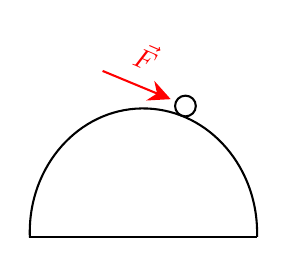
\begin{tikzpicture}[x=0.75pt,y=0.75pt,yscale=-1,xscale=1]
%uncomment if require: \path (0,300); %set diagram left start at 0, and has height of 300

%Straight Lines [id:da1116874193876789] 
\draw    (70,240) -- (180,240) ;


%Shape: Arc [id:dp6219200921642993] 
\draw  [draw opacity=0] (70.55,240.31) .. controls (70.53,239.79) and (70.51,239.27) .. (70.5,238.75) .. controls (69.99,205.7) and (94.09,178.54) .. (124.33,178.07) .. controls (154.57,177.6) and (179.51,204) .. (180.02,237.05) .. controls (180.03,238.01) and (180.03,238.97) .. (180,239.92) -- (125.26,237.9) -- cycle ; \draw   (70.55,240.31) .. controls (70.53,239.79) and (70.51,239.27) .. (70.5,238.75) .. controls (69.99,205.7) and (94.09,178.54) .. (124.33,178.07) .. controls (154.57,177.6) and (179.51,204) .. (180.02,237.05) .. controls (180.03,238.01) and (180.03,238.97) .. (180,239.92) ;
%Shape: Circle [id:dp5387201513730098] 
\draw   (140.5,176.9) .. controls (140.5,174.14) and (142.74,171.9) .. (145.5,171.9) .. controls (148.26,171.9) and (150.5,174.14) .. (150.5,176.9) .. controls (150.5,179.66) and (148.26,181.9) .. (145.5,181.9) .. controls (142.74,181.9) and (140.5,179.66) .. (140.5,176.9) -- cycle ;
%Straight Lines [id:da3091034418461407] 
\draw [color={rgb, 255:red, 255; green, 0; blue, 0 }  ,draw opacity=1 ]   (105.6,160) -- (136.55,172.83) ;
\draw [shift={(138.4,173.6)}, rotate = 202.52] [fill={rgb, 255:red, 255; green, 0; blue, 0 }  ,fill opacity=1 ][line width=0.75]  [draw opacity=0] (10.72,-5.15) -- (0,0) -- (10.72,5.15) -- (7.12,0) -- cycle    ;


% Text Node
\draw (126.8,153) node [color={rgb, 255:red, 255; green, 0; blue, 0 }  ,opacity=1 ,rotate=-23.5]  {$\vec{F}$};


\end{tikzpicture}
